\section{Testy rozmytych regulatorów PID}
\label{lab:zad4}

W tym samym programie zaimplementowac rozmyty algorytm PI lub PID. Dla tej samej
trajektorii zmian sygnału wartosci zadanej spróbowac dobrac parametry lokalnych
algorytmów PI (PID) w taki sposób, aby osiagnac lepsza jakosc regulacji w porównaniu
z regulatorem klasycznym (pojedynczym). Wykonac eksperymenty dla 3 regulatorów
lokalnych. Omówic proces doboru parametrów i zamiescic uzyskane przebiegi regulacji.

% \begin{figure}[H] 
%    \centering
%    % This file was created by matlab2tikz.
%
\definecolor{mycolor1}{rgb}{0.00000,0.44700,0.74100}%
\definecolor{mycolor2}{rgb}{0.85000,0.32500,0.09800}%
%
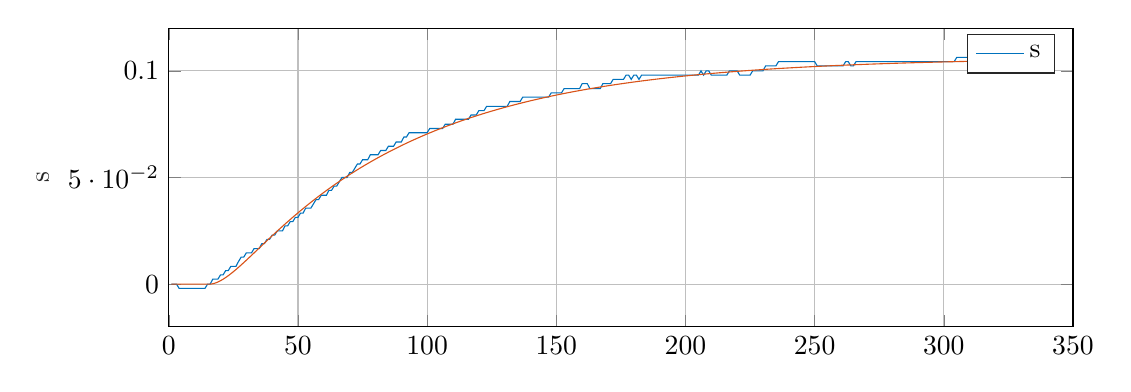
\begin{tikzpicture}

\begin{axis}[%
  width=4.521in,
  height=1.493in,
  at={(0.758in,2.554in)},
scale only axis,
xmin=0,
xmax=350,
ymin=-0.02,
ymax=0.12,
ylabel style={font=\color{white!15!black}},
ylabel={s},
axis background/.style={fill=white},
xmajorgrids,
ymajorgrids,
legend style={legend cell align=left, align=left, draw=white!15!black}
]
\addplot [color=mycolor1]
  table[row sep=crcr]{%
1	0\\
2	0\\
3	0\\
4	-0.00200000000000008\\
5	-0.00200000000000008\\
6	-0.00200000000000008\\
7	-0.00200000000000008\\
8	-0.00200000000000008\\
9	-0.00200000000000008\\
10	-0.00200000000000008\\
11	-0.00200000000000008\\
12	-0.00200000000000008\\
13	-0.00200000000000008\\
14	-0.00200000000000008\\
15	0\\
16	0\\
17	0.00233333333333334\\
18	0.00233333333333334\\
19	0.00233333333333334\\
20	0.00433333333333342\\
21	0.00433333333333342\\
22	0.00633333333333326\\
23	0.00633333333333326\\
24	0.00833333333333333\\
25	0.00833333333333333\\
26	0.00833333333333333\\
27	0.0106666666666667\\
28	0.0126666666666668\\
29	0.0126666666666668\\
30	0.0146666666666666\\
31	0.0146666666666666\\
32	0.0146666666666666\\
33	0.0166666666666667\\
34	0.0166666666666667\\
35	0.0166666666666667\\
36	0.019\\
37	0.019\\
38	0.0210000000000001\\
39	0.0210000000000001\\
40	0.0229999999999999\\
41	0.0229999999999999\\
42	0.025\\
43	0.025\\
44	0.025\\
45	0.0273333333333333\\
46	0.0273333333333333\\
47	0.0293333333333334\\
48	0.0293333333333334\\
49	0.0313333333333333\\
50	0.0313333333333333\\
51	0.0333333333333333\\
52	0.0333333333333333\\
53	0.0356666666666667\\
54	0.0356666666666667\\
55	0.0356666666666667\\
56	0.0376666666666668\\
57	0.0396666666666666\\
58	0.0396666666666666\\
59	0.0416666666666667\\
60	0.0416666666666667\\
61	0.0416666666666667\\
62	0.044\\
63	0.044\\
64	0.0460000000000001\\
65	0.0460000000000001\\
66	0.0479999999999999\\
67	0.05\\
68	0.05\\
69	0.05\\
70	0.0523333333333333\\
71	0.0523333333333333\\
72	0.0543333333333334\\
73	0.0563333333333333\\
74	0.0563333333333333\\
75	0.0583333333333333\\
76	0.0583333333333333\\
77	0.0583333333333333\\
78	0.0606666666666667\\
79	0.0606666666666667\\
80	0.0606666666666667\\
81	0.0606666666666667\\
82	0.0626666666666667\\
83	0.0626666666666667\\
84	0.0626666666666667\\
85	0.0646666666666666\\
86	0.0646666666666666\\
87	0.0646666666666666\\
88	0.0666666666666667\\
89	0.0666666666666667\\
90	0.0666666666666667\\
91	0.069\\
92	0.069\\
93	0.0710000000000001\\
94	0.0710000000000001\\
95	0.0710000000000001\\
96	0.0710000000000001\\
97	0.0710000000000001\\
98	0.0710000000000001\\
99	0.0710000000000001\\
100	0.0710000000000001\\
101	0.0729999999999999\\
102	0.0729999999999999\\
103	0.0729999999999999\\
104	0.0729999999999999\\
105	0.0729999999999999\\
106	0.0729999999999999\\
107	0.075\\
108	0.075\\
109	0.075\\
110	0.075\\
111	0.0773333333333333\\
112	0.0773333333333333\\
113	0.0773333333333333\\
114	0.0773333333333333\\
115	0.0773333333333333\\
116	0.0773333333333333\\
117	0.0793333333333334\\
118	0.0793333333333334\\
119	0.0793333333333334\\
120	0.0813333333333333\\
121	0.0813333333333333\\
122	0.0813333333333333\\
123	0.0833333333333333\\
124	0.0833333333333333\\
125	0.0833333333333333\\
126	0.0833333333333333\\
127	0.0833333333333333\\
128	0.0833333333333333\\
129	0.0833333333333333\\
130	0.0833333333333333\\
131	0.0833333333333333\\
132	0.0856666666666667\\
133	0.0856666666666667\\
134	0.0856666666666667\\
135	0.0856666666666667\\
136	0.0856666666666667\\
137	0.0876666666666668\\
138	0.0876666666666668\\
139	0.0876666666666668\\
140	0.0876666666666668\\
141	0.0876666666666668\\
142	0.0876666666666668\\
143	0.0876666666666668\\
144	0.0876666666666668\\
145	0.0876666666666668\\
146	0.0876666666666668\\
147	0.0876666666666668\\
148	0.0896666666666666\\
149	0.0896666666666666\\
150	0.0896666666666666\\
151	0.0896666666666666\\
152	0.0896666666666666\\
153	0.0916666666666667\\
154	0.0916666666666667\\
155	0.0916666666666667\\
156	0.0916666666666667\\
157	0.0916666666666667\\
158	0.0916666666666667\\
159	0.0916666666666667\\
160	0.094\\
161	0.094\\
162	0.094\\
163	0.0916666666666667\\
164	0.0916666666666667\\
165	0.0916666666666667\\
166	0.0916666666666667\\
167	0.0916666666666667\\
168	0.094\\
169	0.094\\
170	0.094\\
171	0.094\\
172	0.0960000000000001\\
173	0.0960000000000001\\
174	0.0960000000000001\\
175	0.0960000000000001\\
176	0.0960000000000001\\
177	0.0979999999999999\\
178	0.0979999999999999\\
179	0.0960000000000001\\
180	0.0979999999999999\\
181	0.0979999999999999\\
182	0.0960000000000001\\
183	0.0979999999999999\\
184	0.0979999999999999\\
185	0.0979999999999999\\
186	0.0979999999999999\\
187	0.0979999999999999\\
188	0.0979999999999999\\
189	0.0979999999999999\\
190	0.0979999999999999\\
191	0.0979999999999999\\
192	0.0979999999999999\\
193	0.0979999999999999\\
194	0.0979999999999999\\
195	0.0979999999999999\\
196	0.0979999999999999\\
197	0.0979999999999999\\
198	0.0979999999999999\\
199	0.0979999999999999\\
200	0.0979999999999999\\
201	0.0979999999999999\\
202	0.0979999999999999\\
203	0.0979999999999999\\
204	0.0979999999999999\\
205	0.0979999999999999\\
206	0.1\\
207	0.0979999999999999\\
208	0.1\\
209	0.1\\
210	0.0979999999999999\\
211	0.0979999999999999\\
212	0.0979999999999999\\
213	0.0979999999999999\\
214	0.0979999999999999\\
215	0.0979999999999999\\
216	0.0979999999999999\\
217	0.1\\
218	0.1\\
219	0.1\\
220	0.1\\
221	0.0979999999999999\\
222	0.0979999999999999\\
223	0.0979999999999999\\
224	0.0979999999999999\\
225	0.0979999999999999\\
226	0.1\\
227	0.1\\
228	0.1\\
229	0.1\\
230	0.1\\
231	0.102333333333333\\
232	0.102333333333333\\
233	0.102333333333333\\
234	0.102333333333333\\
235	0.102333333333333\\
236	0.104333333333333\\
237	0.104333333333333\\
238	0.104333333333333\\
239	0.104333333333333\\
240	0.104333333333333\\
241	0.104333333333333\\
242	0.104333333333333\\
243	0.104333333333333\\
244	0.104333333333333\\
245	0.104333333333333\\
246	0.104333333333333\\
247	0.104333333333333\\
248	0.104333333333333\\
249	0.104333333333333\\
250	0.104333333333333\\
251	0.102333333333333\\
252	0.102333333333333\\
253	0.102333333333333\\
254	0.102333333333333\\
255	0.102333333333333\\
256	0.102333333333333\\
257	0.102333333333333\\
258	0.102333333333333\\
259	0.102333333333333\\
260	0.102333333333333\\
261	0.102333333333333\\
262	0.104333333333333\\
263	0.104333333333333\\
264	0.102333333333333\\
265	0.102333333333333\\
266	0.104333333333333\\
267	0.104333333333333\\
268	0.104333333333333\\
269	0.104333333333333\\
270	0.104333333333333\\
271	0.104333333333333\\
272	0.104333333333333\\
273	0.104333333333333\\
274	0.104333333333333\\
275	0.104333333333333\\
276	0.104333333333333\\
277	0.104333333333333\\
278	0.104333333333333\\
279	0.104333333333333\\
280	0.104333333333333\\
281	0.104333333333333\\
282	0.104333333333333\\
283	0.104333333333333\\
284	0.104333333333333\\
285	0.104333333333333\\
286	0.104333333333333\\
287	0.104333333333333\\
288	0.104333333333333\\
289	0.104333333333333\\
290	0.104333333333333\\
291	0.104333333333333\\
292	0.104333333333333\\
293	0.104333333333333\\
294	0.104333333333333\\
295	0.104333333333333\\
296	0.104333333333333\\
297	0.104333333333333\\
298	0.104333333333333\\
299	0.104333333333333\\
300	0.104333333333333\\
301	0.104333333333333\\
302	0.104333333333333\\
303	0.104333333333333\\
304	0.104333333333333\\
305	0.106333333333333\\
306	0.106333333333333\\
307	0.106333333333333\\
308	0.106333333333333\\
309	0.106333333333333\\
310	0.106333333333333\\
311	0.106333333333333\\
312	0.106333333333333\\
313	0.106333333333333\\
314	0.106333333333333\\
315	0.106333333333333\\
316	0.106333333333333\\
};
\addlegendentry{s}

\addplot [color=mycolor2, forget plot]
  table[row sep=crcr]{%
1	0\\
2	0\\
3	0\\
4	0\\
5	0\\
6	0\\
7	0\\
8	0\\
9	0\\
10	0\\
11	0\\
12	0\\
13	0\\
14	0\\
15	0\\
16	0\\
17	0.000185072726593913\\
18	0.000529762157235997\\
19	0.00101179142541201\\
20	0.00161166986027936\\
21	0.00231234854140959\\
22	0.00309891837973291\\
23	0.00395834547506707\\
24	0.00487923914863741\\
25	0.00585164861702559\\
26	0.00686688477189672\\
27	0.00791736396630322\\
28	0.00899647109093682\\
29	0.0100984395590469\\
30	0.011218246112695\\
31	0.0123515186206803\\
32	0.0134944552643298\\
33	0.0146437537053256\\
34	0.0157965490032791\\
35	0.0169503592028822\\
36	0.0181030376438027\\
37	0.0192527311633722\\
38	0.0203978434645666\\
39	0.0215370030115851\\
40	0.0226690348940507\\
41	0.0237929361698612\\
42	0.0249078542571998\\
43	0.0260130679992361\\
44	0.0271079710715184\\
45	0.0281920574427976\\
46	0.0292649086357297\\
47	0.0303261825652036\\
48	0.0313756037594771\\
49	0.032412954793356\\
50	0.0334380687837283\\
51	0.0344508228162469\\
52	0.0354511321881499\\
53	0.0364389453664071\\
54	0.0374142395728253\\
55	0.0383770169186555\\
56	0.0393273010208055\\
57	0.0402651340401466\\
58	0.0411905740897459\\
59	0.0421036929673015\\
60	0.0430045741716982\\
61	0.0438933111685524\\
62	0.0447700058739529\\
63	0.0456347673294039\\
64	0.0464877105443123\\
65	0.0473289554852807\\
66	0.0481586261940279\\
67	0.0489768500180066\\
68	0.0497837569397504\\
69	0.0505794789927122\\
70	0.0513641497528626\\
71	0.0521379038966476\\
72	0.052900876817061\\
73	0.0536532042906086\\
74	0.0543950221888332\\
75	0.0551264662288497\\
76	0.055847671758028\\
77	0.0565587735685614\\
78	0.0572599057381829\\
79	0.0579512014937577\\
80	0.0586327930948822\\
81	0.0593048117349739\\
82	0.0599673874576511\\
83	0.0606206490864698\\
84	0.0612647241663269\\
85	0.0618997389150483\\
86	0.0625258181838602\\
87	0.06314308542561\\
88	0.0637516626697359\\
89	0.0643516705031151\\
90	0.0649432280560237\\
91	0.0655264529925401\\
92	0.0661014615048034\\
93	0.0666683683106152\\
94	0.0672272866539331\\
95	0.0677783283078643\\
96	0.0683216035798122\\
97	0.0688572213184768\\
98	0.0693852889224439\\
99	0.0699059123501322\\
100	0.0704191961308975\\
101	0.0709252433771164\\
102	0.0714241557970963\\
103	0.0719160337086766\\
104	0.0724009760534037\\
105	0.0728790804111772\\
106	0.0733504430152778\\
107	0.0738151587676982\\
108	0.0742733212547111\\
109	0.0747250227626123\\
110	0.0751703542935904\\
111	0.0756094055816759\\
112	0.0760422651087328\\
113	0.0764690201204589\\
114	0.0768897566423643\\
115	0.0773045594957058\\
116	0.0777135123133523\\
117	0.0781166975555663\\
118	0.0785141965256825\\
119	0.0789060893856721\\
120	0.0792924551715803\\
121	0.0796733718088276\\
122	0.0800489161273669\\
123	0.0804191638766892\\
124	0.0807841897406728\\
125	0.0811440673522712\\
126	0.0814988693080356\\
127	0.0818486671824703\\
128	0.0821935315422174\\
129	0.08253353196007\\
130	0.0828687370288128\\
131	0.0831992143748894\\
132	0.0835250306718956\\
133	0.0838462516538994\\
134	0.0841629421285881\\
135	0.0844751659902422\\
136	0.0847829862325382\\
137	0.0850864649611807\\
138	0.0853856634063644\\
139	0.0856806419350687\\
140	0.0859714600631851\\
141	0.0862581764674798\\
142	0.086540848997392\\
143	0.0868195346866712\\
144	0.0870942897648534\\
145	0.08736516966858\\
146	0.0876322290527585\\
147	0.08789552180157\\
148	0.088155101039323\\
149	0.0884110191411563\\
150	0.0886633277435924\\
151	0.0889120777549443\\
152	0.0891573193655763\\
153	0.0893991020580219\\
154	0.0896374746169588\\
155	0.0898724851390461\\
156	0.0901041810426215\\
157	0.0903326090772639\\
158	0.0905578153332212\\
159	0.0907798452507056\\
160	0.0909987436290584\\
161	0.091214554635786\\
162	0.0914273218154689\\
163	0.0916370880985449\\
164	0.0918438958099695\\
165	0.0920477866777536\\
166	0.0922488018413815\\
167	0.0924469818601101\\
168	0.0926423667211514\\
169	0.0928349958477398\\
170	0.0930249081070853\\
171	0.0932121418182153\\
172	0.0933967347597051\\
173	0.0935787241773002\\
174	0.0937581467914312\\
175	0.0939350388046215\\
176	0.0941094359087925\\
177	0.0942813732924642\\
178	0.0944508856478553\\
179	0.0946180071778825\\
180	0.0947827716030618\\
181	0.0949452121683118\\
182	0.0951053616496615\\
183	0.0952632523608638\\
184	0.0954189161599146\\
185	0.0955723844554814\\
186	0.0957236882132403\\
187	0.0958728579621239\\
188	0.0960199238004813\\
189	0.0961649154021507\\
190	0.096307862022447\\
191	0.0964487925040645\\
192	0.0965877352828966\\
193	0.0967247183937732\\
194	0.0968597694761176\\
195	0.0969929157795227\\
196	0.0971241841692502\\
197	0.0972536011316501\\
198	0.0973811927795059\\
199	0.0975069848573026\\
200	0.0976310027464219\\
201	0.0977532714702629\\
202	0.0978738156992915\\
203	0.0979926597560179\\
204	0.0981098276199045\\
205	0.0982253429322042\\
206	0.0983392290007302\\
207	0.0984515088045595\\
208	0.0985622049986688\\
209	0.0986713399185062\\
210	0.0987789355844975\\
211	0.0988850137064893\\
212	0.0989895956881299\\
213	0.0990927026311872\\
214	0.0991943553398074\\
215	0.0992945743247118\\
216	0.0993933798073359\\
217	0.0994907917239092\\
218	0.0995868297294779\\
219	0.0996815132018709\\
220	0.0997748612456094\\
221	0.0998668926957619\\
222	0.0999576261217444\\
223	0.100047079831068\\
224	0.10013527187303\\
225	0.100222220042362\\
226	0.100307941882812\\
227	0.10039245469069\\
228	0.100475775518359\\
229	0.100557921177669\\
230	0.100638908243356\\
231	0.100718753056383\\
232	0.100797471727238\\
233	0.100875080139185\\
234	0.100951593951466\\
235	0.101027028602466\\
236	0.101101399312823\\
237	0.1011747210885\\
238	0.101247008723818\\
239	0.101318276804432\\
240	0.101388539710282\\
241	0.101457811618491\\
242	0.101526106506224\\
243	0.101593438153512\\
244	0.101659820146031\\
245	0.10172526587784\\
246	0.10178978855409\\
247	0.101853401193683\\
248	0.101916116631899\\
249	0.10197794752299\\
250	0.10203890634273\\
251	0.102099005390932\\
252	0.102158256793932\\
253	0.102216672507033\\
254	0.102274264316922\\
255	0.10233104384404\\
256	0.102387022544936\\
257	0.102442211714572\\
258	0.102496622488605\\
259	0.102550265845633\\
260	0.102603152609411\\
261	0.102655293451034\\
262	0.102706698891089\\
263	0.102757379301781\\
264	0.102807344909024\\
265	0.102856605794503\\
266	0.10290517189771\\
267	0.10295305301795\\
268	0.103000258816316\\
269	0.103046798817641\\
270	0.103092682412416\\
271	0.10313791885869\\
272	0.103182517283934\\
273	0.103226486686883\\
274	0.103269835939355\\
275	0.103312573788036\\
276	0.10335470885625\\
277	0.103396249645694\\
278	0.103437204538157\\
279	0.103477581797211\\
280	0.103517389569877\\
281	0.103556635888268\\
282	0.103595328671213\\
283	0.10363347572585\\
284	0.103671084749208\\
285	0.103708163329752\\
286	0.10374471894892\\
287	0.103780758982632\\
288	0.103816290702776\\
289	0.103851321278675\\
290	0.103885857778536\\
291	0.103919907170877\\
292	0.103953476325926\\
293	0.103986572017019\\
294	0.104019200921953\\
295	0.104051369624347\\
296	0.104083084614958\\
297	0.104114352293001\\
298	0.104145178967433\\
299	0.104175570858228\\
300	0.104205534097637\\
301	0.104235074731415\\
302	0.10426419872005\\
303	0.104292911939964\\
304	0.104321220184694\\
305	0.104349129166065\\
306	0.104376644515342\\
307	0.104403771784368\\
308	0.104430516446677\\
309	0.104456883898609\\
310	0.104482879460389\\
311	0.104508508377208\\
312	0.104533775820276\\
313	0.104558686887868\\
314	0.104583246606353\\
315	0.104607459931206\\
316	0.104631331748012\\
};
\end{axis}
\end{tikzpicture}%
%    \caption{Punkt pracy obiektu symulacji}
%    \label{projekt:zad1:figure:charstat_u_y_z}
% \end{figure}

\subsection{Funkcja przynależności}
\label{lab:zad4:fuzzyFunction}


\newpage

\subsection{Implementacja rozmytego algorytmu PID}
\label{lab:zad4:implPID}


\newpage

\subsection{Dobór parametrów lokalnych regulatorów PID}
\label{lab:zad4:paramPID}

\newpage
